The graph shows the spectrum of an X-ray tube: a continuous part (bremsstrahlung) and two sharp lines. The table lists the lines of three anode materials.

\begin{center}
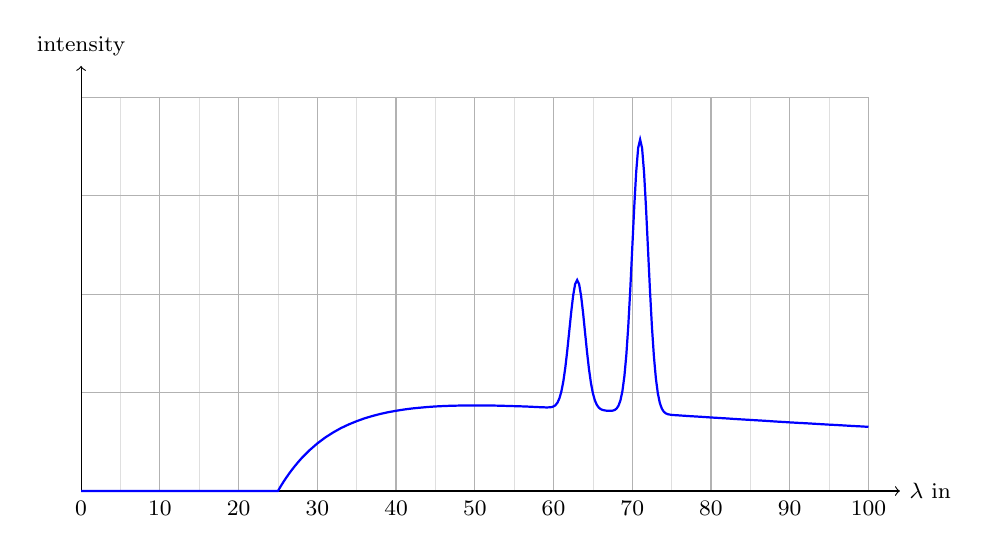
\begin{tikzpicture}[font=\footnotesize]
 \draw[gray!25, very thin] (0.500,0) -- (0.500,5.000) (1.500,0) -- (1.500,5.000) (2.500,0) -- (2.500,5.000) (3.500,0) -- (3.500,5.000) (4.500,0) -- (4.500,5.000) (5.500,0) -- (5.500,5.000) (6.500,0) -- (6.500,5.000) (7.500,0) -- (7.500,5.000) (8.500,0) -- (8.500,5.000) (9.500,0) -- (9.500,5.000);
 \draw[gray!60, thin] (0.000,0) -- (0.000,5.000) (1.000,0) -- (1.000,5.000) (2.000,0) -- (2.000,5.000) (3.000,0) -- (3.000,5.000) (4.000,0) -- (4.000,5.000) (5.000,0) -- (5.000,5.000) (6.000,0) -- (6.000,5.000) (7.000,0) -- (7.000,5.000) (8.000,0) -- (8.000,5.000) (9.000,0) -- (9.000,5.000) (10.000,0) -- (10.000,5.000);
 \draw[gray!60, thin] (0,0.000) -- (10.000,0.000) (0,1.250) -- (10.000,1.250) (0,2.500) -- (10.000,2.500) (0,3.750) -- (10.000,3.750) (0,5.000) -- (10.000,5.000);
 \node[below] at (0.000,0) {0};
 \node[below] at (1.000,0) {10};
 \node[below] at (2.000,0) {20};
 \node[below] at (3.000,0) {30};
 \node[below] at (4.000,0) {40};
 \node[below] at (5.000,0) {50};
 \node[below] at (6.000,0) {60};
 \node[below] at (7.000,0) {70};
 \node[below] at (8.000,0) {80};
 \node[below] at (9.000,0) {90};
 \node[below] at (10.000,0) {100};
 \draw[->] (0,0) -- (10.400,0) node[right] {$\lambda$ in \si{\pico\meter}};
 \draw[->] (0,0) -- (0,5.400) node[above] {intensity};
 \draw[thick, blue] plot coordinates {(0.000,0.000) (0.100,0.000) (0.200,0.000) (0.300,0.000) (0.400,0.000) (0.500,0.000) (0.600,0.000) (0.700,0.000) (0.800,0.000) (0.900,0.000) (1.000,0.000) (1.100,0.000) (1.200,0.000) (1.300,0.000) (1.400,0.000) (1.500,0.000) (1.600,0.000) (1.700,0.000) (1.800,0.000) (1.900,0.000) (2.000,0.000) (2.100,0.000) (2.200,0.000) (2.300,0.000) (2.325,0.000) (2.350,0.000) (2.375,0.000) (2.400,0.000) (2.425,0.000) (2.450,0.000) (2.475,0.000) (2.500,0.000) (2.525,0.043) (2.550,0.084) (2.575,0.123) (2.600,0.161) (2.625,0.197) (2.650,0.232) (2.675,0.266) (2.700,0.298) (2.725,0.329) (2.750,0.359) (2.775,0.388) (2.800,0.416) (2.900,0.517) (3.000,0.604) (3.100,0.679) (3.200,0.743) (3.300,0.799) (3.400,0.846) (3.500,0.887) (3.600,0.923) (3.700,0.953) (3.800,0.979) (3.900,1.001) (4.000,1.019) (4.100,1.035) (4.200,1.048) (4.300,1.058) (4.400,1.067) (4.500,1.074) (4.600,1.079) (4.700,1.083) (4.800,1.085) (4.900,1.087) (5.000,1.087) (5.100,1.087) (5.200,1.086) (5.300,1.084) (5.400,1.081) (5.500,1.078) (5.600,1.075) (5.700,1.071) (5.800,1.066) (5.825,1.065) (5.850,1.064) (5.875,1.063) (5.900,1.062) (5.925,1.062) (5.950,1.063) (5.975,1.066) (6.000,1.074) (6.025,1.090) (6.050,1.122) (6.075,1.177) (6.100,1.265) (6.125,1.394) (6.150,1.569) (6.175,1.787) (6.200,2.031) (6.225,2.275) (6.250,2.487) (6.275,2.630) (6.300,2.680) (6.325,2.627) (6.350,2.481) (6.375,2.267) (6.400,2.019) (6.425,1.772) (6.450,1.552) (6.475,1.374) (6.500,1.242) (6.525,1.152) (6.550,1.094) (6.575,1.059) (6.600,1.040) (6.625,1.029) (6.650,1.024) (6.675,1.020) (6.700,1.019) (6.725,1.018) (6.750,1.021) (6.775,1.028) (6.800,1.046) (6.825,1.083) (6.850,1.151) (6.875,1.269) (6.900,1.456) (6.925,1.731) (6.950,2.103) (6.975,2.565) (7.000,3.083) (7.025,3.603) (7.050,4.052) (7.075,4.357) (7.100,4.464) (7.125,4.354) (7.150,4.045) (7.175,3.593) (7.200,3.070) (7.225,2.549) (7.250,2.084) (7.275,1.709) (7.300,1.430) (7.325,1.240) (7.350,1.119) (7.375,1.048) (7.400,1.008) (7.425,0.987) (7.450,0.976) (7.475,0.971) (7.500,0.967) (7.525,0.965) (7.550,0.963) (7.575,0.962) (7.600,0.960) (7.625,0.958) (7.650,0.957) (7.675,0.955) (7.700,0.953) (7.800,0.947) (7.900,0.941) (8.000,0.934) (8.100,0.928) (8.200,0.922) (8.300,0.915) (8.400,0.909) (8.500,0.903) (8.600,0.897) (8.700,0.891) (8.800,0.884) (8.900,0.878) (9.000,0.872) (9.100,0.866) (9.200,0.861) (9.300,0.855) (9.400,0.849) (9.500,0.843) (9.600,0.838) (9.700,0.832) (9.800,0.826) (9.900,0.821) (10.000,0.815)};
\end{tikzpicture}
\end{center}

\begin{center}
\begin{tabular}{lccc}
 anode & copper & molybdenum & silver \\ \hline
 $K_\alpha$ & \SI{154}{\pico\m} & \SI{71}{\pico\m} & \SI{56}{\pico\m} \\
 $K_\beta$ & \SI{139}{\pico\m} & \SI{63}{\pico\m} & \SI{50}{\pico\m}
\end{tabular}
\end{center}

\begin{abcliste}
\abc Read off the shortest wavelength in the spectrum.

\abc Calculate the voltage of the tube.

\abc What is the anode made of?
\end{abcliste}
